

%------------------------------------------------------------------------
\section{Serving Two Masters: Stability and Diversity with RpGAN \texorpdfstring{$+ R_1+R_2$}{R-1R-2}}
%---An Improved Training Objective \vk{title can be tweaked; i recommend naming your new loss}}
% James Tompkin: I wrote 'serving two masters'. Note that 'serving two masters' is inherently a religious label; in the bible, Matthew writes that one cannot serve two masters (only God). In the traditions of monarchy (to which our title alludes in the procession of kings), a king had divine right and so avoided this problem of serving two masters (to serve God and to serve one's king is to serve two masters, except once we establish that kings are divine then this problem goes away as the same master - God - is then being served). I am not religious.
\label{sec:loss}

In defining a GAN objective, we tackle two challenges: stability and diversity. Some previous work deals with stability~\cite{sg1,sg2,sg3} and other previous work deals with mode collapse \cite{rgan}. To make progress in both, we combine a stable method with a simple regularizer that is grounded by theory.


\subsection{Traditional GAN}
A traditional GAN~\cite{gan,nowozin2016f} is formulated as a minimax game between a discriminator (or critic) $D_\psi$ and a generator $G_\theta$. Given real data $x\sim p_\mathcal{D}$ and fake data $x\sim p_\theta$ produced by $G_\theta$, the most general form of a GAN is given by:
\begin{align}
\begin{split}
\label{eq:gan}
\mathcal{L}(\theta,\psi)=\mathbb{E}_{z\sim p_z}\left[f\left(  D_\psi(G_\theta(z))\right)\right]+\mathbb{E}_{x\sim p_\mathcal{D}}\left[f\left( -D_\psi(x) \right)\right]
\end{split}
\end{align}
\noindent where $G$ tries to minimize $\mathcal{L}$ while $D$ tries to maximize it. The choice of $f$ is flexible~\cite{lsgan,hingegan}. In particular, $f(t) = -\log(1+e^{-t})$ recovers the classic GAN by Goodfellow~\etal~\cite{gan}. For the rest of this work, this will be our choice of $f$~\cite{nowozin2016f}.

% It is shown that Eq.\ref{eq:gan} is actually convex if we can directly optimize $p_\theta$~\cite{gan,rpgan}. Though in practice, the empirical GAN loss moves fake samples past the decision boundary induced by $D$ rather than updating the density function $p_\theta$ directly. This turns out to be a much harder problem that is susceptible to two common failure cases: mode collapse/dropping\footnote{Mode collapse and mode dropping are technically two related yet distinct problems. We use these two terms interchangeably hereafter to refer to the general problem where $\supp p_\theta$ fails to fully cover $\supp p_\mathcal{D}$.} and non-convergence. \vk{Minor thing: could provide a bit more information (1 sentence) on mode dropping and collapse}
It has been shown that Equation~\ref{eq:gan} has convex properties when $p_\theta$ can be optimized directly~\cite{gan,rpgan}. However, in practical implementations, the empirical GAN loss typically shifts fake samples beyond the decision boundary set by $D$, as opposed to directly updating the density function $p_\theta$. This deviation leads to a significantly more challenging problem, characterized by susceptibility to two prevalent failure scenarios: mode collapse/dropping\footnote{While mode collapse and mode dropping are technically distinct issues, they are used interchangeably in this context to describe the common problem where $\supp(p_\theta)$ does not comprehensively cover $\supp(p_\mathcal{D})$. Mode collapse refers to the generator producing a limited diversity of samples (i.e., one image for the entire distribution), whereas mode dropping involves the generator failing to represent certain modes of the data distribution (ignoring entire subsets of the training distribution).} and non-convergence.



\subsection{Relativistic \texorpdfstring{$f$-GAN}{f-GAN}}
% We adopt relativistic pairing GAN (RpGAN) by Jolicoeur-Martineau~\etal~\cite{rgan} as the main GAN loss. 
% Sun~\etal showed that RpGAN is especially effective against mode dropping~\cite{rpgan} as the loss landscape of RpGAN contains no local minima that correspond to mode dropping solutions. 
% Next, we apply zero-centered gradient penalties~\cite{r1,r1r2} to RpGAN. Gradient penalty is a well known technique that stabilizes GAN training~\cite{wgan-gp,r1r2,r1} and has been proven to be crucial to GAN convergence~\cite{r1}. As our contribution to the theory, we follow Mescheder~\etal~\cite{r1} and prove that gradient-penalized RpGAN enjoys the same guarantee of local convergence as regularized classic GANs. In addition to theoretical guarantees, our empirical results suggest that gradient penalized RpGAN is sufficiently well-behaved, to the extent that allows us to remove all GAN tricks without encountering non-convergence or mode dropping.

We employ a slightly different minimax game named relativistic pairing GAN (RpGAN) by Jolicoeur-Martineau~\etal~\cite{rgan} to address mode dropping. The general RpGAN is defined as:
\begin{equation}
\label{eq:rpgan}
\mathcal{L}(\theta,\psi)=\mathbb{E}_{\substack{z\sim p_z\\x\sim p_\mathcal{D}}}\left[f\left(  D_\psi(G_\theta(z))-D_\psi(x) \right)\right]
\end{equation}
Although Eq.~\ref{eq:rpgan} differs only slightly from Eq.~\ref{eq:gan}, evaluating this critic difference has a fundamental impact on the landscape of $\mathcal{L}$. Since Eq.~\ref{eq:gan} merely requires $D$ to separate real and fake data, in the scenario where all real and fake data can be separated by a single decision boundary, the empirical GAN loss encourages $G$ to simply move all fake samples barely past this single boundary---this degenerate solution is what we observe as mode collapse/dropping. Sun~\etal~\cite{rpgan} characterize such degenerate solutions as bad local minima in the landscape of $\mathcal{L}$, and show that Eq.~\ref{eq:gan} has \emph{exponentially many} bad local minima. The culprit is the existence of a single decision boundary that naturally arises when real and fake data are considered in isolation. RpGAN introduces a simple solution by coupling real and fake data,~\ie a fake sample is critiqued by its realness \emph{relative to} a real sample, which effectively maintains a decision boundary in the neighborhood of \emph{each} real sample and hence forbids mode dropping. Sun~\etal~\cite{rpgan} show that the landscape of Eq.~\ref{eq:rpgan} contains no local minima that correspond to mode dropping solutions, and that every basin is a global minimum.


\subsection{Training Dynamics of RpGAN}
Although the RpGAN landscape result~\cite{rpgan} allows us to address mode dropping, the training dynamics of RpGAN have yet to be studied. The ultimate goal of Eq.~\ref{eq:rpgan} is to find the equilibrium $(\theta^*,\psi^*)$ such that $p_{\theta^*}=p_\mathcal{D}$ and $D_{\psi^*}$ is constant everywhere on $p_\mathcal{D}$. Sun~\etal~\cite{rpgan} show that $\theta^*$ is globally reachable along a non-increasing trajectory in the landscape of Eq.~\ref{eq:rpgan} under reasonable assumptions. However, the existence of such a trajectory does not necessarily mean that gradient descent will find it. Jolicoeur-Martineau~\etal show empirically that unregularized RpGAN does not perform well~\cite{rgan}. 

\vspace{1ex}
\noindent \textbf{Proposition~\upperRomannumeral{1}.} (Informal) \emph{Unregularized RpGAN does not always converge using gradient descent.}
%\vk{Propositions should ideally be made precise or in the worst case, say it's an informal statement (but then you still have to make it intuitively understandable)}
\vspace{1ex}

\noindent We confirm this proposition with a proof in Appendix B. 
% In summary, we follow Mescheder~\etal~\cite{r1} and inherit their DiracGAN counterexample to apply it to RpGAN. 
We show analytically that RpGAN does not converge for certain types of $p_\mathcal{D}$, such as ones that approach a delta distribution. Thus, further regularization is necessary to fill in the missing piece of a well-behaved loss.

\paragraph{Zero-centered gradient penalties.}
To tackle RpGAN non-convergence, we explore gradient penalties as the solution since it is proven that zero-centered gradient penalties (0-GP) facilitate convergent training for classic GANs~\cite{r1}. The two most commonly-used 0-GPs are $R_1$ and $R_2$:
\begin{equation}
\begin{aligned}
R_1(\psi)&=\frac{\gamma}{2}\mathbb{E}_{x\sim p_\mathcal{D}}\left[\left\| \nabla_x D_\psi \right \|^2\right]\\ 
R_2(\theta,\psi)&=\frac{\gamma}{2}\mathbb{E}_{x\sim p_\theta}\hspace{0.06cm}\left[\left\| \nabla_x D_\psi \right \|^2\right]
\end{aligned}
\end{equation}
$R_1$ penalizes the gradient norm of $D$ on real data, and $R_2$ penalizes the gradient norm of $D$ on fake data. Analysis on the training dynamics of GANs has thus far focused on local convergence~\cite{nagarajan2017gradient,gannum,r1},~\ie, whether the training at least converges when $(\theta,\psi)$ are in a neighborhood of $(\theta^*,\psi^*)$. In such a scenario, the convergence behavior can be analyzed~\cite{nagarajan2017gradient,gannum,r1} by examining the spectrum of the Jacobian of the gradient vector field $\left(-\nabla_\theta\mathcal{L},\nabla_\psi\mathcal{L} \right )$ at $(\theta^*,\psi^*)$. The key insight here is that when $G$ already produces the true distribution, we want $\nabla_x D=0$, so that $G$ is not pushed away from its optimal state, and thus the training does not oscillate. $R_1$ and $R_2$ impose such a constraint when $p_\theta=p_\mathcal{D}$. This also explains why earlier attempts at gradient penalties, such as the one-centered gradient penalty (1-GP) in WGAN-GP~\cite{wgan-gp}, fail to achieve convergent training~\cite{r1} as they still encourage $D$ to have a non-zero slope when $G$ has reached optimality.

Since the same insight also applies to RpGAN, 
we extend our previous analysis and show that:
% our goal is to extend the proof of Mescheder~\etal~\cite{r1} to RpGAN and show that:

\vspace{1ex}
\noindent \textbf{Proposition~\upperRomannumeral{2}.} (Informal) \emph{RpGAN with $R_1$ or $R_2$ regularization is locally convergent subject to similar assumptions as in} Mescheder~\etal~\cite{r1}.
\vspace{1ex}

In Appendix C, our proof similarly analyzes the eigenvalues of the Jacobian of the regularized RpGAN gradient vector field at $(\theta^*,\psi^*)$. We show that all eigenvalues have a negative real part; thus, regularized RpGAN is convergent in a neighborhood of $(\theta^*,\psi^*)$ for small enough learning rates~\cite{r1}.

%\vk{This paragraph is too verbose and feels like belongs to a prior work or discussion section} 
\paragraph{Discussion.}
Another line of work~\cite{r1r2} links $R_1$ and $R_2$ to instance noise~\cite{instancenoise} as its analytical approximation. Roth et al.~\cite{r1r2} showed that for the classic GAN~\cite{gan} by Goodfellow~\etal, $R_1$ approximates convolving $p_\mathcal{D}$ with the density function of $\mathcal{N}(0, \gamma I)$, up to additional weighting and a Laplacian error term. $R_2$ likewise approximates convolving $p_\theta$ with $\mathcal{N}(0, \gamma I)$ up to similar error terms. The Laplacian error terms from $R_1$, $R_2$ cancel when $D_\psi$ approaches $D_{\psi^*}$. We do not extend Roth~\etal's proof~\cite{r1r2} to RpGAN; however, this approach might provide complimentary insights to our work, which follows the strategy of Mescheder~\etal~\cite{r1}.

\subsection{A Practical Demonstration}

%\vk{i don't think that the rest of this section belongs in the methods section; i would first make it less verbose, then i would move large parts of it to the experiments, and i would summarize here in 1-2 sentences} 

We experiment with how well-behaved our loss is on StackedMNIST~\cite{pacgan} which consists of 1000 uniformly-distributed modes. The network is a small ResNet~\cite{resnet2} for $G$ and $D$ without any normalization layers~\cite{bn,gn,ln,in}.
Through the use of a pretrained MNIST classifier, we can explicitly measure how many modes of $p_\mathcal{D}$ are recovered by $p_\theta$. Furthermore, we can estimate the reverse KL divergence between the fake and real samples $D_\text{KL}\left(p_\theta\parallel p_\mathcal{D} \right)$ via the KL divergence between the categorical distribution of $p_\theta$ and the true uniform distribution.
\begin{figure}
\begin{floatrow}
\ffigbox{%
  \centering
  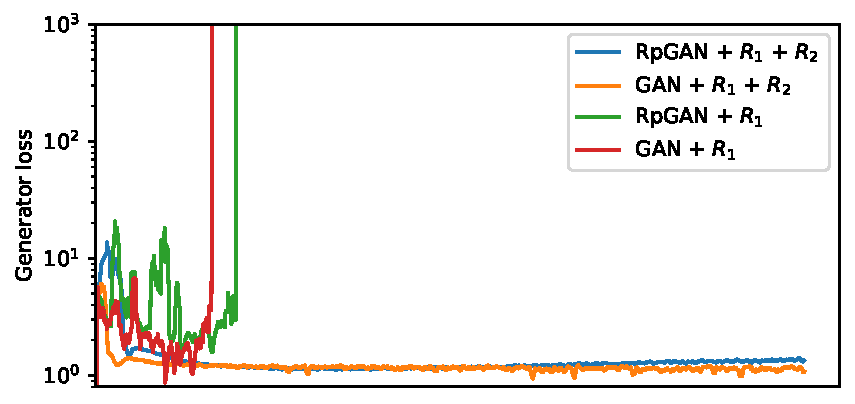
\includegraphics[width=0.48\textwidth]{figures/MNIST_loss.pdf}%
}{%
\caption{Generator $G$ loss for different objectives over training. Regardless of which objective is used, training diverges with only $R_1$ and succeeded with both $R_1$ and $R_2$. Convergence failure with only $R_1$ was noted by Lee et al.~\cite{vitgan}.}
\label{fig:mnist_loss_curve}
}
\capbtabbox{%
\centering
    \begin{tabular}{ l rrr }
        \toprule
        Loss & \# modes$\uparrow$ & $D_\text{KL}$$\downarrow$ \\
        \midrule
        RpGAN $+ R_1+R_2$ & $\mathbf{1000}$ & $\mathbf{0.0781}$ \\
        GAN $+ R_1+R_2$ & $693$ & $0.9270$ \\
        RpGAN $+ R_1$ & Fail & Fail \\
        GAN $+ R_1$ & Fail & Fail \\
        \bottomrule
    \end{tabular}
}{%
    \caption{StackedMNIST~\cite{pacgan} result for each loss function. The maximum possible mode coverage is 1000. ``Fail'' indicates that training diverged early on.}
    \label{tab:loss}
}
\end{floatrow}
\end{figure}

%For our initial experiments, we adopt a small ResNet~\cite{resnet2} architecture without any normalization layer~\cite{bn,gn,ln,in} for $G$ and $D$. 
A conventional GAN loss with $R_1$, as used by Mescheder et al.~\cite{r1} and the StyleGAN series~\cite{sg1, sg2, sg3}, diverges quickly (Fig.~\ref{fig:mnist_loss_curve}). Next, while theoretically sufficient for local convergence, RpGAN with only $R_1$ regularization is also unstable and diverges quickly\footnote{Varying $\gamma$ from 0.1 to 100 does not stabilize training.}. In each case, the gradient of $D$ on fake samples explodes when training diverges. With both $R_1$ and $R_2$, training becomes stable for both the classic GAN and RpGAN. Now stable, we can see that the classic GAN suffers from mode dropping, whereas RpGAN achieves full mode coverage (Tab.~\ref{tab:loss}) and reduces $D_\text{KL}$ from 0.9270 to 0.0781. As a point of contrast, StyleGAN~\cite{sg1,sg2,sg2ada,sg3} uses the minibatch standard deviation trick to reduce mode dropping, improving mode coverage from 857 to 881 on StackedMNIST\footnote{These numbers are from Karras~\etal~\cite{pggan}, Table 4. "857" corresponds to a low-capacity version of a progressive GAN and "881" adds the minibatch standard deviation trick. Further comparisons via loss curves are difficult since progressive GAN is a substantially different model than the small ResNet we use for this experiment.} and with barely any improvement on $D_\text{KL}$~\cite{pggan}.

%With training instability out of our way, we are ready to examine quantitatively how our new loss performs compared to existing work~\cite{r1,pggan,sg2}. While with $R_1$ and $R_2$ in conjunction training is successful for both the classic GAN~\cite{gan} and RpGAN~\cite{rgan}, we see in Table~\ref{tab:loss} that the classic GAN suffers from mode dropping. In contrast, RpGAN not only achieves full mode coverage, more notably, it drastically reduces $D_\text{KL}$ from 0.927 to 0.0781, indicating a considerably more faithful reconstruction of $p_\mathcal{D}$. 

% Instead of modifying the loss function, the StyleGAN family~\cite{sg1,sg2,sg2ada,sg3} relies on a trick called minibatch standard deviation~\cite{pggan} to combat mode dropping. It is shown in~\cite{pggan} that minibatch standard deviation can only slightly improve mode coverage from 857 to 881 on StackedMNIST and it shows barely any improvement on $D_\text{KL}$. 
% RpGAN in comparison improves mode coverage from 693 to 1000 and reduces $D_\text{KL}$ by one magnitude. 
%This shows that RpGAN is not only more principled against mode dropping in theory, but more effective in practice too. 
% We show in Section.\ref{sec:exp} that with architectural improvements in Section.\ref{sec:roadmap}, we can further improve $D_\text{KL}$ on StackedMNIST and even beat likelihood-based models. For the rest of this work, RpGAN $+ R_1+R_2$ will be our loss function.

% We start with RpGAN with only $R_1$ regularization since theoretically this is sufficient for local convergence. Contrary to our expectations, the training process utilizing this loss function exhibited significant instability and rapidly diverged. We experimented with various values of $\gamma$, ranging from 0.1 to 100; however, none succeeded in stabilizing the training. Furthermore, we explored integrating the conventional GAN loss combined with $R_1$, as commonly employed in the work of Mescheder et al.~\cite{r1} and the StyleGAN series~\cite{sg1, sg2, sg3}. Notably, this configuration led to even quicker divergence than the $R_1$ regularized RpGAN.
%To our surprise, training with this loss has been quite unstable and it diverges very quickly. We tried different $\gamma$ values ranging from 0.1 to 100 but none could prevent training from diverging. We also experiment with the combination of classic GAN and $R_1$, this is the widely adopted GAN loss in Mescheder~\etal~\cite{r1} and the StyleGAN family~\cite{sg1,sg2,sg3}, yet this loss diverges even faster than $R_1$ regularized RpGAN. 

% Upon closer inspection, we notice that the gradient of $D$ on fake samples explodes when training diverges. This motivates us to also apply $R_2$ regularization along with $R_1$, we see in Figure~\ref{fig:mnist_loss_curve} that with both $R_1$ and $R_2$, training becomes stable for both the classic GAN and RpGAN. 

$R_1$ alone is not sufficient for globally-convergent training. While a theoretical analysis of this is difficult, our small demonstration still provides insights into the assumptions of our convergence proof. 
In particular, the assumption that $(\theta,\psi)$ are sufficiently close to $(\theta^*,\psi^*)$ is highly unlikely early in training. In this scenario, if $D$ is sufficiently powerful, regularizing $D$ solely on real data is not likely to have much effect on $D$'s behavior on fake data and so training can fail due to an ill-behaved $D$ on fake data. This observation has been made by previous studies~\cite{r1gradexp, r1gradexpcvpr} specifically for empirical GAN training, that regularizing an empirical discriminator with only $R_1$ leads to gradient explosion on fake data due to the memorization of real samples.

% \vk{this is the key part that should be summarized in 1-2 sentences in this section: you find empirically and mathematically that both types of regularization are needed to make things work; then in the experiments section or in the appendix you provide results that show that it's the case}

Thus, the practical solution is to regularize $D$ on both real and fake data. The benefit of doing so can be viewed from the insight of Roth~\etal~\cite{r1r2}: that applying $R_1$ and $R_2$ in conjunction smooths both $p_\mathcal{D}$ and $p_\theta$ which makes learning easier than only smoothing $p_\mathcal{D}$. We also find empirically that with both $R_1$ and $R_2$ in place, $D$ tends to satisfy $\mathbb{E}_{x\sim p_\mathcal{D}}\left[\left\| \nabla_x D \right \|^2\right]\approx\mathbb{E}_{x\sim p_\theta}\left[\left\| \nabla_x D \right \|^2\right]$ even early in the training. Jolicoeur-Martineau~\etal~\cite{ganmmc} show that in this case $D$ becomes a maximum margin classifier---but if only one regularization term is applied, this does not hold. Additionally, having roughly the same gradient norm on real and fake data potentially reduces discriminator overfitting, as Fang~\etal~\cite{diggan} observe that the gradient norm on real and fake data diverges when $D$ starts to overfit.

% \vk{by the way, you will need a discussion of your regularization to other uses of this similar regularizer in the discussion or related work section}